\chapter{Einleitung}
\section{Umfang}
Dieses Dokument enthält eine Sammlung von Konzepten und Best Practices ausgelegt auf KMUs.\\

Das Dokument reicht von sehr abstrakten Konzepten bis zu konkreten Best Practices.
Der Guide ist so generell und herstellerunabhängig als möglich gehalten.
Bei defacto Standards in der KMU IT-Landschaft, gibt es kleine Anleitungen zur Bedienung oder Konfiguration des Produktes.
Der Guide fokussiert sich auf Open-Source Software soweit möglich und realistisch.\\

Dieser Guide sollte für KMUs der entsprechenden Grösse in der Matrix relevant sein.

\begin{table}[H]
    \begin{center}
        \begin{tabular}{l|c|c|c}
            Guide                & mikro KMU & kleines KMU & mittleres KMU\\
            \hline
            Geräteverschlüsslung & X         & X             & X\\
            \acrlong{av}         & X         & X             & X\\
            Backup               & X         & X             & X\\
            Updates \& Patching  & O         & X             & X\\
            Firewall             & O         & X             & X\\
            \acrfull{iam}        &           & X             & X\\
            \acrfull{laps}       &           & O             & X\\
        \end{tabular}
        \caption*{X = starke Empfehlung, O = Empfehlung}
    \end{center}
    \caption{Guiderelevanz entsprechend KMU Grösse}
\end{table}

\begin{figure}[H]
    \centering
    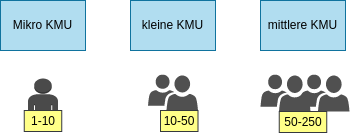
\includegraphics[width=0.6\linewidth]{../img/kmu.png}
    \caption{Einteilung KMU Grössen}
\end{figure}

\section{Ausgewählte Themen}
Die ausgewählten Themen sind alles wichtige Bestandteile, die von Firmen umgesetzt werden um die Sicherheit in der IT-Infrastruktur zu erhöhen.
Die Themen wurden aus folgenden Gründen gewählt:

\begin{itemize}
    \item \textbf{Geräteverschlüsselung}: Physische Sicherheit bei Diebstahl oder Verlust.
    \item \textbf{\acrlong{av}}: Sicherheit bei Viren und Malware.
    \item \textbf{Backup}: Recovery bei Verlust oder Ransomware.
    \item \textbf{Updates \& Patching}: Fortlaufende Sicherheit bei neuen Attacken.
    \item \textbf{Firewall}: Sicherheit zwischen Netzwerken und gegen aussen.
    \item \textbf{\acrshort{iam}}: Zugriffskontrolle und Verwaltung. Sicherheit vor Datendiebstahl.
    \item \textbf{\acrshort{laps}}: Sicherheit vor Verbreitung bei komprimierten Geräten.
\end{itemize}